%%%%%%%%%%%%%%%%%%%%%%%%%%%%%%%%%%%%%%%%%
% Engineering Calculation Paper
% LaTeX Template
% Version 1.0 (20/1/13)
%
% This template has been downloaded from:
% http://www.LaTeXTemplates.com
%
% Original author:
% Dmitry Volynkin (dim_voly@yahoo.com.au)
%
% License:
% CC BY-NC-SA 3.0 (http://creativecommons.org/licenses/by-nc-sa/3.0/)
%
% Modificaciones por Roberto Cerdas
%
% Si desea utilizar notas al margen, favor leer los comentarios en las líneas 32 y % 52. Si desea colocar un logo, favor leer comentario en línea 54. El comando     % \marginnote{texto} introduce notas al margen.  
%
%%%%%%%%%%%%%%%%%%%%%%%%%%%%%%%%%%%%%%%%%

%----------------------------------------------------------------------------------------
%	PACKAGES AND OTHER DOCUMENT CONFIGURATIONS
%----------------------------------------------------------------------------------------

\documentclass[12pt,a4paper]{article} % Use A4 paper with a 12pt font size - different paper sizes will require manual recalculation of page margins and border positions

\usepackage[spanish]{babel} % Utilizar reglas de idioma español
\usepackage[utf8]{inputenc} % Use UTF-8 encoding
\usepackage{marginnote} % Required for margin notes
\usepackage{wallpaper} % Required to set each page to have a background
\usepackage{lastpage} % Required to print the total number of pages
%\usepackage[left=1.3cm,right=4.6cm,top=1.8cm,bottom=4.0cm,marginparwidth=3.4cm]{geometry} % Comentar la línea abajo y descomentar esta para usar notas al margen
\usepackage[left=1.3cm,right=1.3cm,top=1.8cm,bottom=4.0cm]{geometry} % Adjust page margins
\usepackage{amsmath} % Required for equation customization
\usepackage{amssymb} % Required to include mathematical symbols
\usepackage{xcolor} % Required to specify colors by name
\usepackage[square, comma, sort&compress]{natbib} % Use the natbib reference package - read up on this to edit the reference style; if you want text (e.g. Smith et al., 2012) for the in-text references (instead of numbers), remove 'numbers' 

\usepackage{fancyhdr} % Required to customize headers
\setlength{\headheight}{80pt} % Increase the size of the header to accommodate meta-information
\pagestyle{fancy}\fancyhf{} % Use the custom header specified below
\renewcommand{\headrulewidth}{0pt} % Remove the default horizontal rule under the header

\setlength{\parindent}{0cm} % Remove paragraph indentation
\newcommand{\tab}{\hspace*{2em}} % Defines a new command for some horizontal space

\newcommand\BackgroundStructure{ % Command to specify the background of each page
\setlength{\unitlength}{1mm} % Set the unit length to millimeters

\setlength\fboxsep{0mm} % Adjusts the distance between the frameboxes and the borderlines
\setlength\fboxrule{0.5mm} % Increase the thickness of the border line
\put(10, 10){\fcolorbox{black}{white!10}{\framebox(192,247){}}} % Main content box
%\put(165, 10){\fcolorbox{black}{blue!10}{\framebox(37,247){}}} % Margin box: Descomentar para utilizar notas al margen.
\put(10, 262){\fcolorbox{black}{white!10}{\framebox(192, 25){}}} % Header box
%\put(143, 263){\includegraphics[height=23mm,keepaspectratio]{logo}} % Logo box - maximum height/width: 25x42. Descomentar esta línea para usar logo.
}

%----------------------------------------------------------------------------------------
%	HEADER INFORMATION
%----------------------------------------------------------------------------------------

\fancyhead[L]{\begin{tabular}{l r | l r} % The header is a table with 4 columns
\textbf{Proyecto} & Diseño flip-flop CMOS & \textbf{Página} & \thepage/\pageref{LastPage} \\ % Project name and page count
\textbf{Trabajo} & Proceso de diseño & \textbf{Actualizado en:} & 31/10/2015 \\ % Job number and last updated date
\textbf{Curso} & VLSI & \textbf{Revisado en:} & 2/11/2015 \\ % Version and reviewed date
\textbf{Diseñador} & López F. - Quirós.J.& \textbf{Revisado por:} & Alfonso Chacón Rodríguez \\ % Designer and reviewer
\end{tabular}}

%----------------------------------------------------------------------------------------

\begin{document}



\AddToShipoutPicture{\BackgroundStructure} % Set the background of each page to that specified above in the header information section

%----------------------------------------------------------------------------------------
%	DOCUMENT CONTENT
%----------------------------------------------------------------------------------------


\section{Resumen} 

En este documento se presentan los resultados del diseño de un registro flip-flop en una tecnología ON Semiconductor 0.5 $\mu$m, el cual se caracterizó y se midieron sus valores de tiempo mas importantes. Tambien se presenta las respuesta a las preguntas de teoriía sobre los valores de tiempo en un registro flip-flop y sobre las diferencias entre los flip-flop estáticos y dinámicos.

\section{Introducción} 

El flip-flop es un tipo de circuito secuencial, capaz almacenar un valor lógico a partir de su entrada en un flanco de señal de reloj. Esta señal perdura durante el periodo de la señal de reloj hasta el proximo flanco de subida o de bajada, dependiendo de su fabricación. Idealmente, el tiempo requerido para el almacenamiento de información es cero, pero a como veremos a continuación, dependerá de la tecnología con la que se ha constrido el flip-flop que habrán tiempos que se deberán respetar para que su funcionamiento sea el esperado.

Para este documento se iniciará dando una breve explicación acerca de lo que son los tiempos que estarán definidos para el diseño del flip-flop incluidos los tiempos de propagación de la señales. Luego se explicarán acerca de lo que son los registros estáticos y dinamico, asi como las ventajas y desventajas que poseen cada uno, esto con el fin de observar el potencial que poseen cada uno en diversas aplicaciones.

También se mostrará en este documento, el diseño en layout de un flip-flop master-slave para 1 bit en tecnología ON-semiconductor 0.5 $\mu$m. asi como las consideraciones que se tomaron para el mismo.

Por último se mostrará las simulaciones que se realizaron para la caracterización del flip-flop y medición de los valores de tiempos del mismo.

\section{Definición de conceptos}

\begin{itemize}
\item Set-up time: Es el tiempo mínimo el cual debe tener la entrada D antes del flanco de reloj, para que sea un valor válido de entrada y pueda ser cargado en el flip-flop. 
Para el circuito propuesto, esta propagación es medible por los tiempos de propagación que requiere los transistores del bloque Master, esto antes del flanco de reloj y que se empiece a propagar la entrada en el bloque Slave. De no ser así los valores de los buffers de salida del bloque no se traslapen y den un valor incorrecto. 
El valor de set-up en un flip-flop master salve es el mostrado en la ecuación (), esta viene de que la entrada debe propagarse en 3 inversores y en 1 buffer de paso:
 $3 *tpd_inv + tpd_tx$

\item Hold time: Es el tiempo mínimo el cual se debe mantener el valor de entrada D, luego del flanco de reloj, para que sea un válido que se pueda cargar en el flip-flop.
Para el circuito propuesto, este valor es cero. Esto porque al haberse dado el flanco de reloj, el transistor de paso en la entrada en el bloque Master se cierra por lo que el valor de entrada a partir de ese momento no afectará en lo absoluto a la salida. 

\item Tiempo de propagación: Es el tiempo que le toma al flip-flop en el peor caso, para tener un valor válido de salida igual al valor cargado leído en la entrada.
En el Flip-Flop Master-Slave, este tiempo es el cual le tomará la salida del bloque master propagarse en el bloque Slave. Para ello solo le tomará el tiempo de propagación de un inversor y de un buffer de paso, ya que se consideró en el setup-time el tiempo para el transistor de entrada del bloque.
Este valor se puede calcular con la ecuación (): 

$tpd_tx + tpd_inv.$

\item Tiempo de contaminación: Es el menor tiempo que le toma al flip-flop para tener un valor de salida igual al valor de la entrada que se había leído anteriormente.

\end{itemize}

\section{Flip-Flops estáticos y dinámicos}


La función logica a la que se le realizara el trazado y el Diagrama de Palitos es la mostrada en la Ec.\ref{eqn:logica}. Esta función lógica es conocida como $OAI-22 + INV.$ Para el diseno de la compuerta se utilizó algebra booleana y se obtuvo la Ec.\ref{eqn:logica_inversa}.

\begin{equation}\label{eqn:logica}
F=(A+B)*(C+D)
\end{equation}

\begin{equation}\label{eqn:logica_inversa}
\overline{F}=\overline{(A+B)}+\overline{(C+D)}
\end{equation}\\


Para lo cual se hizo el esquemático mostrado en la \textit{Fig.\ref{fig:Comp_Transistores}} y se hizo el \textit{Diagrama de Palitos} mostrado en la \textit{Fig.\ref{fig:inv_est}}. En este diagrama se dibujaron tanto la compuerta \textit{OAI22} como el \textit{Inversor} para cambiar el nivel lógico a la salida, por lo que se observa mas de una tira de difusión en la parte inferior, resultado de la inclusión del \textit{Inversor} en el diagrama.\\

\begin{figure}[htbp]
  \centering
    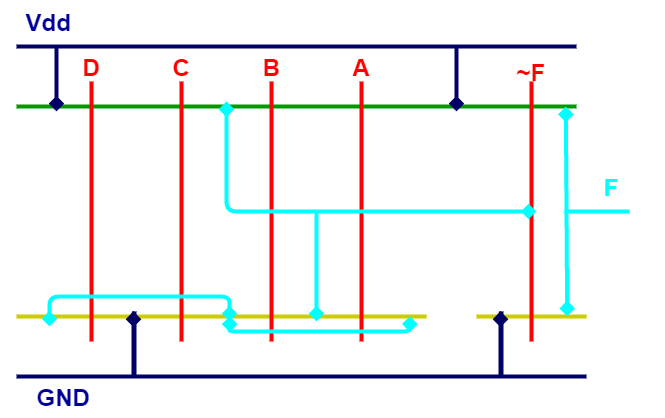
\includegraphics[scale=0.4]{./Palitos.png}
    \rule{35em}{0.5pt}
  \caption[IdealvsSim]{Diagrama de palitos de la función OAI22 + INV}
  \label{fig:pal}
\end{figure}

\section{Diseño del layout}

\subsection{Bloque Master}

El cálculo de los tiempos de propagación y de contaminación se realiza haciendo uso de dos métodos: la teoría del esfuerzo lógico, \textit{logical effort}, y por el método de la aproximación de Elmore, \textit{Elmore Delay}.\\

\subsection{Inversor en el Master}

El esfuerzo lógico se define como \textit{"la razón de la capacitancia del gate a la capacitancia de entrada de un inversor que puede entregar la misma corriente de salida."}, e indica que tan mala es una compuerta produciendo una corriente de salida comparada con un inversor.\\

Para el cálculo del delay por medio de la teoría de esfuerzo lógico, se utilizan las formulas del cálculo del delay en redes lógicas con multiples etapas, \textit{Multistage Logical Network}, que utiliza las siguientes formulas para el cálculo del delay:\\

\begin{equation}\label{eqn:esfuerzo_logico}
G= \prod g_{i}
\end{equation}

\begin{equation}\label{eqn:esfuerzo_electrico}
H= \frac{C_{out-path}}{C_{in-path}}
\end{equation}

\begin{equation}\label{eqn:esfuerzo_enramado}
B= \prod b_{i}
\end{equation}

\begin{equation}\label{eqn:esfuerzo}
F = GBH
\end{equation}

\begin{equation}\label{eqn:delay_parasitico}
P = \sum p_{i}
\end{equation}

\begin{equation}\label{eqn:delay}
D = NF^{\frac{1}{N}} + P
\end{equation}

En donde \textit{G} es el esfuerzo lógico, \textit{H} es el esfuerzo eléctrico, \textit{B} el esfuerzo de enramado, \textit{F} es el esfuerzo total, \textit{P} es el delay parasítico del camino, \textit{N} es la cantidad de estapas del camino y \textit{D} es el delay total del camino.\\

La función \textit{F=(A+B)(C+D)} se puede representar a nivel de compuerta como se muestra en la \textit{Fig.\ref{fig:OAI21}} , donde se observa que la compuerta es del tipo OR-OR-AND-INV + INVERSOR, \textit{OAI-21 + inverter}, y a partir de aqui se calcula el esfuerzo lógico de camino.\\

\begin{figure}[htbp]
  \centering
    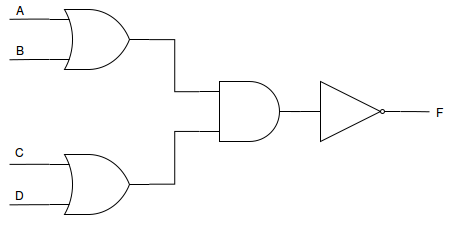
\includegraphics[scale=0.5]{./OAI21.png}
    \rule{35em}{0.5pt}
  \caption[IdealvsSim]{Compuerta \textit{OAI-21}.}
  \label{fig:OAI21}
\end{figure}

Para realizar los cálculos del esfuerzo de camino de esta función, se debe tomar en cuenta que cada entrada presenta como maximo 30$\lambda$ de ancho de transistor, y que la salida debe de manejar una carga equivalente de 500$\lambda$ de ancho de transistor, como se muestra en la \textit{Fig.\ref{fig:OAI21_Cargas}}. Se puede observar que en este caso el número de etapas, \textit{N}, es igual a 2, por lo que haciendo uso de las ecuaciones \textit{\ref{eqn:esfuerzo_logico}, \ref{eqn:esfuerzo_electrico}, \ref{eqn:esfuerzo_enramado}, \ref{eqn:esfuerzo}, \ref{eqn:delay_parasitico}, \ref{eqn:delay}}, se puede encontrar el delay mediante la teoría de esfuerzo lógico de cada entrada bajo estas condiciones de carga.\\

\begin{figure}[htbp]
  \centering
    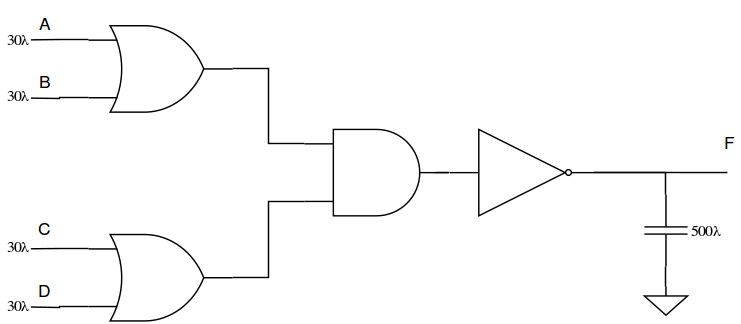
\includegraphics[scale=0.4]{./OAI21_Cargas.png}
    \rule{35em}{0.5pt}
  \caption[IdealvsSim]{Compuerta \textit{OAI-21} con Carga.}
  \label{fig:OAI21_Cargas}
\end{figure}


\begin{equation}\label{eqn:esfuerzo_logico2}
G= \prod g_{i}= \frac{6}{3} * 1 = \frac{6}{3}
\end{equation}

\begin{equation}\label{eqn:esfuerzo_electrico2}
H= \frac{C_{out-path}}{C_{in-path}} = \frac{500\lambda}{30\lambda} = \frac{50}{3}
\end{equation}

\begin{equation}\label{eqn:esfuerzo_enramado2}
B= \prod b_{i} = 1
\end{equation}

\begin{equation}\label{eqn:esfuerzo2}
F = GBH = \frac{6}{3}*1*\frac{50}{3} = \frac{100}{3}
\end{equation}

\begin{equation}\label{eqn:delay_parasitico2}
P = \sum p_{i} = \frac{12}{3} + 1 = \frac{15}{3} = 5
\end{equation}

\begin{equation}\label{eqn:delay2}
D = NF^{\frac{1}{N}} + P = 2*(\frac{100}{3})^{\frac{1}{2}} + 5 = 16.54\tau
\end{equation}\\

El cálculo de los tiempos arroja como resultado que cada entrada de esta compuerta tendrá un delay de \textit{16.54$\tau$}.\\

Con el valor de delay calculado se puede proceder a dimensionar los transistores que conforman la compuerta. En la \textit{Fig.\ref{fig:Comp_Transistores}} se muestra la compuerta compuesta a nivel de transistores, sin dimensionar.\\

\begin{figure}[htbp]
  \centering
    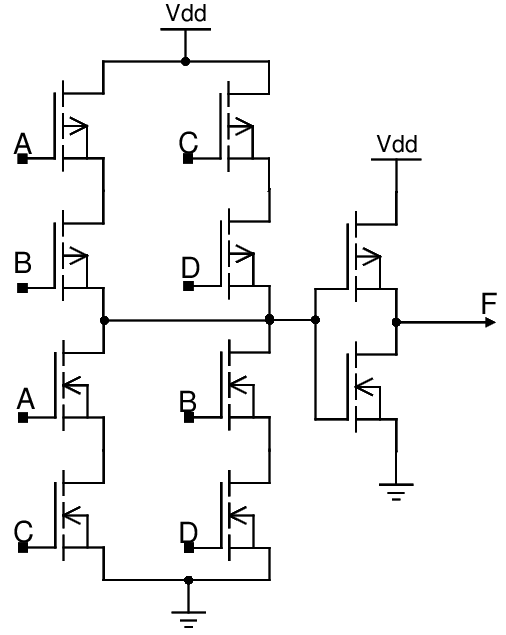
\includegraphics[scale=0.45]{./Comp_Transistores.png}
    \rule{35em}{0.5pt}
  \caption[IdealvsSim]{Esquemático de la Compuerta \textit{F=(A+B)(C+D)} a nivel de transistores sin dimensionar.}
  \label{fig:Comp_Transistores}
\end{figure}

Para dimensionar los transistores de cada entrada, se toma en cuenta el modelo RC del transistor. Sabiendo que la resitencia de la red \textit{PMOS} debe ser igual a la de la red \textit{NMOS}, y que cada entrada presenta como maximo 30$\lambda$ de ancho de transistor se obtiene que:\\

\begin{equation}\label{eqn:R}
\frac{2R}{k_p} = \frac{R}{k_n}
\end{equation}

\begin{equation}\label{eqn:k}
k_p + k_n = 30\lambda
\end{equation}\\

Donde \textit{$k_{p}$} y \textit{$k_{n}$} son los anchos de los tansistores \textit{p} y \textit{n} de cada entrada. Con este sistema de ecuaciones se obtiene que:

\begin{equation}\label{eqn:R1}
k_p = 2k_n
\end{equation}

\begin{equation}\label{eqn:k1}
k_p + k_n = 30\lambda
\end{equation}

\begin{equation}\label{eqn:k2}
3k_n = 30\lambda
\end{equation}

\begin{equation}\label{eqn:k3}
k_n = 10\lambda ; k_p = 20\lambda
\end{equation}\\

Utilizando la \textit{Ec.\ref{eqn:k_Inv}}, se puede encontrar la capacitancia de entrada del inversor, como se muestra a continuación:\\

\begin{equation}\label{eqn:k_Inv}
C_{ini}= \frac{C_{outi}*g_{i}}{F^{\frac{1}{N}}}
\end{equation}

\begin{equation}\label{eqn:k_Inv2}
{C_{in}}_{i}= \frac{500\lambda*1}{5.777} = 86.6\lambda = 87\lambda
\end{equation}\\

Sabiendo que la resistencia en la red de \textit{pull-up} es el doble que la de la red de \textit{pull-down} en el inversor de la salida, se puede encontrar las dimensiones de los anchos de los transistores en dicho inversor.\\

\begin{equation}\label{eqn:k_Inv3}
k_p=2k_n
\end{equation}

\begin{equation}\label{eqn:k_Inv4}
3k_n=87\lambda
\end{equation}

\begin{equation}\label{eqn:k_Inv5}
k_n=29\lambda ; k_p=58\lambda 
\end{equation}\\

En la \textit{Fig.\ref{fig:Comp_Transistores_Dim}} se muestra la compuerta a nivel de transistores, cada uno con su respectivo valor de ancho de canal correspondiente.\\

\begin{figure}[htbp]
  \centering
    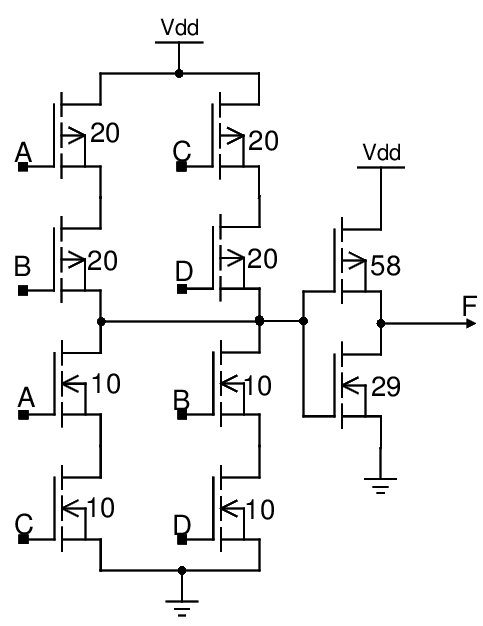
\includegraphics[scale=0.45]{./Comp_Transistores_Dim.png}
    \rule{35em}{0.5pt}
  \caption[Delay]{Esquemático de la Compuerta \textit{F=(A+B)(C+D)} a nivel de transistores con sus respectivas dimensiones, \textit{L=2$\lambda$}.}
  \label{fig:Comp_Transistores_Dim}
\end{figure}

\subsection{Bloque slave}

Ahora se calcula el delay de propagación y el delay de contaminación de la compuerta \textit{F=(A+B)(C+D)} mediante el método de \textit{Aproximación de Elmore}, el cuál se hace valer del modelo RC del transistor, para calcular los delays de una compuerta. El modelo de delay de \textit{Elmore} estima el restraso desde una fuente conmutando a uno de los nodos hoja cambiantes como la suma sobre cada nodo \textit{i} de la capacitancia \textit{$C_{i}$} en el nodo, multiplicado por la resistencia efectiva \textit{$R_{is}$} en el camino compartido desde la fuente hasta el nodo y la hoja, dando como resultado la ec.\ref{eqn:Elmore}:


\begin{equation}\label{eqn:Elmore}
t_{pd} = \sum_{i} R_{is}C_{i}
\end{equation}\\



En la \textit{Fig.\ref{fig:ModeloRC_Completo}} se muestra el modelo \textit{RC} completo de la compuerta, con sus capacitancias y resistencias, para la compuerta \textit{OAI-21} y para el inversor en la salida.\\

\begin{figure}[htbp]
  \centering
    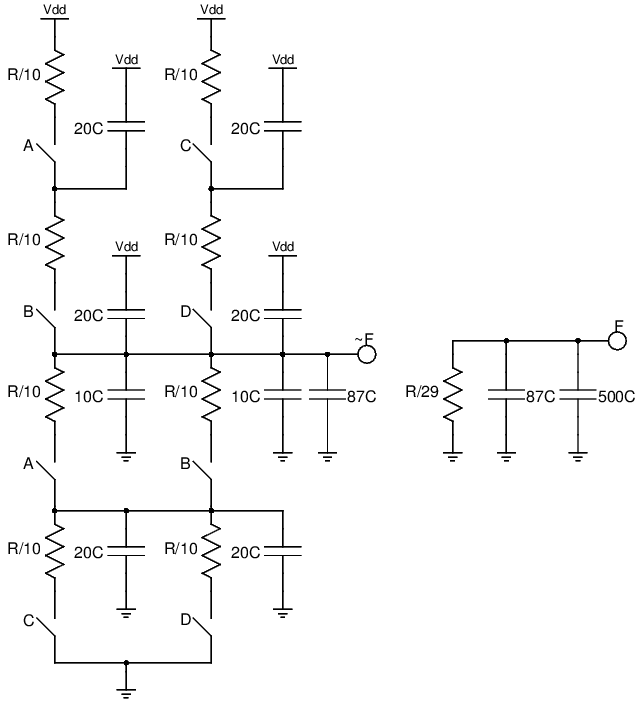
\includegraphics[scale=0.45]{./ModeloRC_Completo.png}
    \rule{35em}{0.5pt}
  \caption[IdealvsSim]{Modelo \textit{RC} completo de la Compuerta \textit{F=(A+B)(C+D)}.}
  \label{fig:ModeloRC_Completo}
\end{figure}

Para este modelo se calculan el mejor y el peor caso para el delay, por lo que en las siguientes secciones se presentaran los cálculos y los circuitos \textit{RC} de cada caso.\\

\subsection{Buffer inversor de salida}

Antes de calcular el mejor y el pesor caso de subida, primero se calcula el retraso provocado por el inversor a la salida, ya que este sera el mismo para el mejor y el peor caso de subida y de bajada. En la \textit{Fig.\ref{fig:RC_Inversor}} se muestra el modelo \textit{RC} del inversor de este problema.\\

\begin{figure}[htbp]
  \centering
    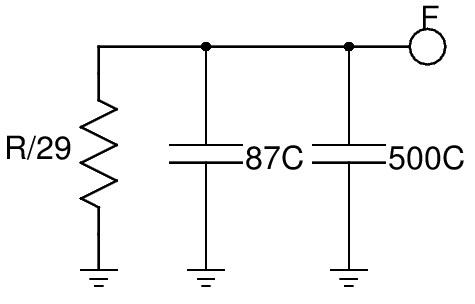
\includegraphics[scale=0.3]{./RC_Inversor.png}
    \rule{35em}{0.5pt}
  \caption[IdealvsSim]{Modelo \textit{RC} del Inversor.}
  \label{fig:RC_Inversor}
\end{figure}

Con este circuito se calcula el delay utilizando la \textit{Ec.\ref{eqn:Elmore_Inv}}, obteniendo como resultado que el delay del inversor para el caso de subida y bajada es:\\

\begin{equation}\label{eqn:Elmore_Inv}
t_{pd} = \frac{R}{29}(500 + 87)C = \frac{587RC}{29} = 20.24RC
\end{equation}\\

Con el delay del inversor calculado en la \textit{Ec.\ref{eqn:Elmore_Inv}}, se procede a realizar los calculos para el mejor y peor caso de delay de subida.\\

En la \textit{Fig.\ref{fig:Mejor_caso_Rise_propagacion}} se observa que el mejor caso ocurre cuando todos los transistores de la red de \textit{pull-up} se encuentran encendidos, o dos transistores están encendidos en la red de \textit{pull-up}, A y B, y los dos transistores mas interiores de la red de \textit{pull-down}, A y B, están apagados, con lo que la red de \textit{pull-down} no contribuye al delay en ambos casos. En la \textit{Ec.\ref{eqn:Elmore_tpdr_Mejor}} se muestra el cálculo del delay para el mejor caso de levantamiento:\\

\begin{figure}[htbp]
  \centering
    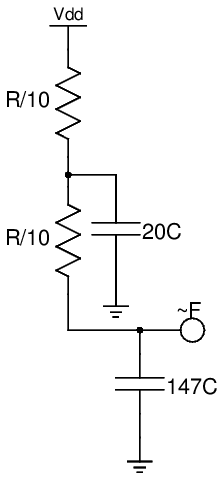
\includegraphics[scale=0.5]{./Mejor_caso_Rise_propagacion.png}
    \rule{35em}{0.5pt}
  \caption[IdealvsSim]{Mejor Caso de \textit{Rise} en el Delay de Propagación.}
  \label{fig:Mejor_caso_Rise_propagacion}
\end{figure}

\begin{equation}\label{eqn:Elmore_tpdr_Mejor}
t_{pdr} = \frac{20RC}{10} + \frac{147*2RC}{10} + t_{pdInv}= 31.4RC + 20.24RC = 51.64RC = 17.213\tau
\end{equation}\\

En la \textit{Fig.\ref{fig:Peor_caso_Rise_propagacion}} se observa que el peor caso ocurre cuando solo dos transistores se encendidos, C y D, y uno o los dos transistores mas interiores de la red de \textit{pull-down} están también encendidos, por lo que la red de \textit{pull-down} contribuye al delay. En la \textit{Ec.\ref{eqn:Elmore_tpdr_Peor}} se muestra el cálculo del delay para el peor caso de levantamiento:\\

\begin{figure}[htbp]
  \centering
    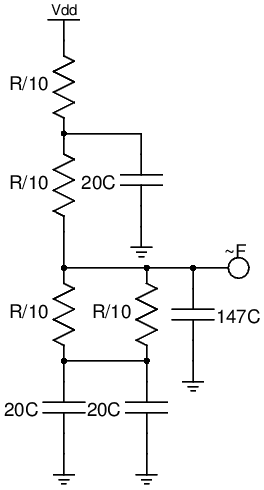
\includegraphics[scale=0.45]{./Peor_caso_Rise_propagacion.png}
    \rule{35em}{0.5pt}
  \caption[IdealvsSim]{Peor Caso de \textit{Rise} en el Delay de Propagación.}
  \label{fig:Peor_caso_Rise_propagacion}
\end{figure}

\begin{equation}\label{eqn:Elmore_tpdr_Peor}
t_{pdr} = \frac{20RC}{10}+\frac{20RC}{5}+\frac{147RC}{5}+t_{pdInv}= 35.4RC + 20.24RC = 55.64RC = 18.546\tau
\end{equation}\\

\subsection{Circuito completo}

En la \textit{Fig.\ref{fig:Peor_caso_Fall_propagacion}} se observa el peor caso de caída en el cálculo del delay en la compuerta. En este caso se activan las entradas A y C, con un 1 lógico, en la red de \textit{pull-down}, y se activan las entradas B y D, con un 0 lógico, en la red de \textit{pull-up}, con lo que esta red contribuye con el delay, tal como se muestra en la \textit{Fig.\ref{fig:Peor_caso_Fall_propagacion}}. En la \textit{Ec.\ref{eqn:Delay_fall_Peor}} se muestra el cálculo del delay.\\

\begin{figure}[htbp]
  \centering
    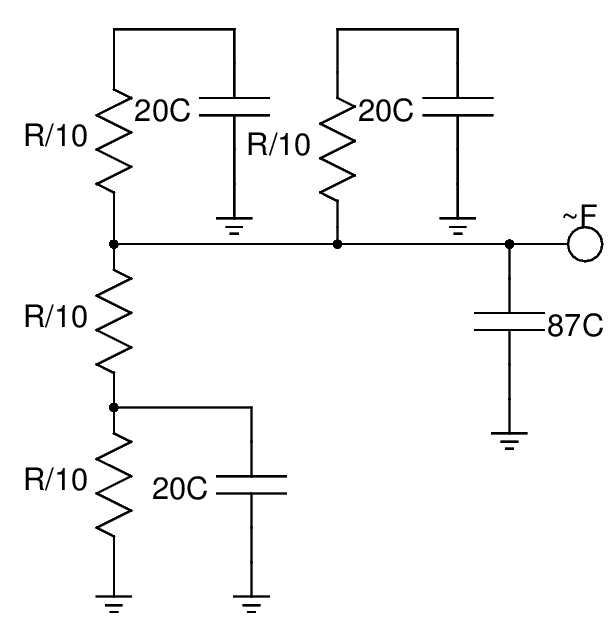
\includegraphics[scale=0.25]{./Peor_caso_Fall_propagacion.png}
    \rule{35em}{0.3pt}
  \caption[C_Carga]{Peor Caso de \textit{Fall} en el Delay de Propagación.}
  \label{fig:Peor_caso_Fall_propagacion}
\end{figure}


\begin{equation}\label{eqn:Delay_fall_Peor}
t_{pdf} = \frac{20RC}{10}+\frac{147RC}{5}+\frac{40RC}{5}+t_{pdInv}=39.4RC+20.24RC=59.64RC=19.88\tau
\end{equation}\\


En la \textit{Fig.\ref{fig:Mejor_caso_Fall_propagacion}} se observa el mejor caso de caída en el cálculo del delay en la compuerta. En este caso se activan las entradas B y D, con un 1 lógico, en la red de \textit{pull-down}, y por ende se desactivan las entradas B y D en la red de \textit{pull-up}, con lo que esta red no contribuye con el delay, tal como se muestra en la \textit{Fig.\ref{fig:Mejor_caso_Fall_propagacion}}. En la \textit{Ec.\ref{eqn:Delay_fall_Mejor}} se muestra el cálculo del delay.\\

\begin{figure}[htbp]
  \centering
    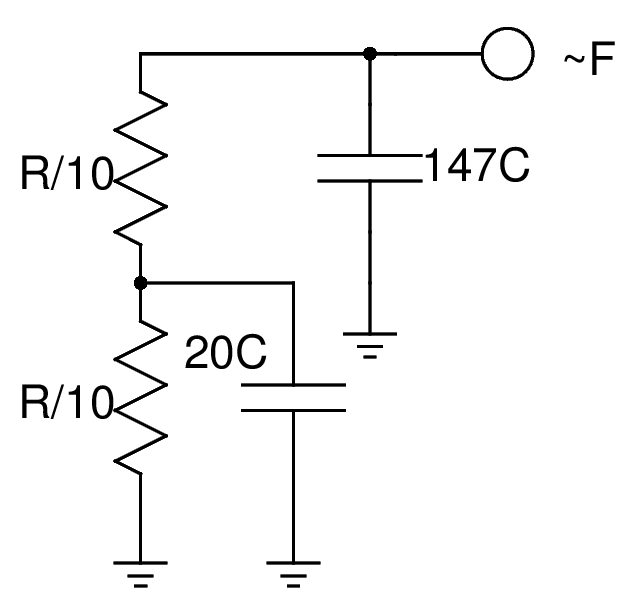
\includegraphics[scale=0.25]{./Mejor_caso_Fall_propagacion.png}
    \rule{35em}{0.3pt}
  \caption[C_Carga]{Mejor Caso de \textit{Fall} en el Delay de Propagación.}
  \label{fig:Mejor_caso_Fall_propagacion}
\end{figure}


\begin{equation}\label{eqn:Delay_fall_Mejor}
t_{pdf} = \frac{20RC}{10}+\frac{147RC}{5}+t_{pdInv}=31.4RC+20.24RC=51.64RC=17.21\tau
\end{equation}\\




\section{Simulación para caracterización del Flip-Flop}

En la figura \ref{fig:layout} se puede observar el diseño del layout de la compuerta de la ecuación \ref{eqn:logica_inversa} en la cual se basó en la figura de palitos de la figura \ref{fig:pal}. En esta se ha usado un "pitch" de $12\lambda$ ya que calza perfectamente con las conexiones para las salidas y entradas así con las conexiones de los metales entre transistores.

También se realizó una simulación del mismo con la rutina que se muestra en la figura \ref{fig:layout_sim} en la cual se simulará el mejor caso para la red de NMOS. El resultado se encuentra en la figura \ref{fig:layout_graf}.

\begin{figure}[htbp]
\begin{center}
    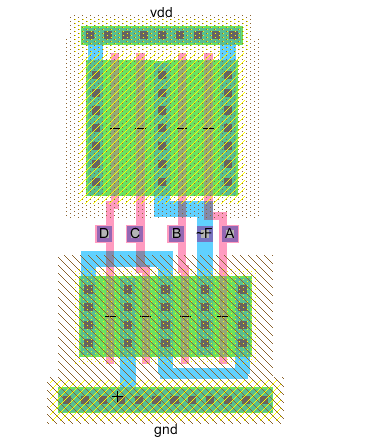
\includegraphics[scale=0.5]{./layout.png}
    \rule{35em}{0.5pt}
  \caption[Captura]{Layout del la $OAI-22$}
  \label{fig:layout}
  \end{center}
\end{figure}

\begin{figure}[htbp]
\begin{center}
    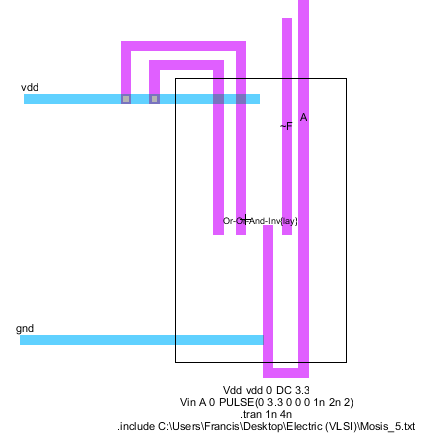
\includegraphics[scale=0.5]{./layout_sim.png}
    \rule{35em}{0.5pt}
  \caption[Captura]{Circuito para simulación en Ltpice del layout del circuito}
  \label{fig:layout_sim}
  \end{center}
\end{figure}

\begin{figure}[htbp]
\begin{center}
    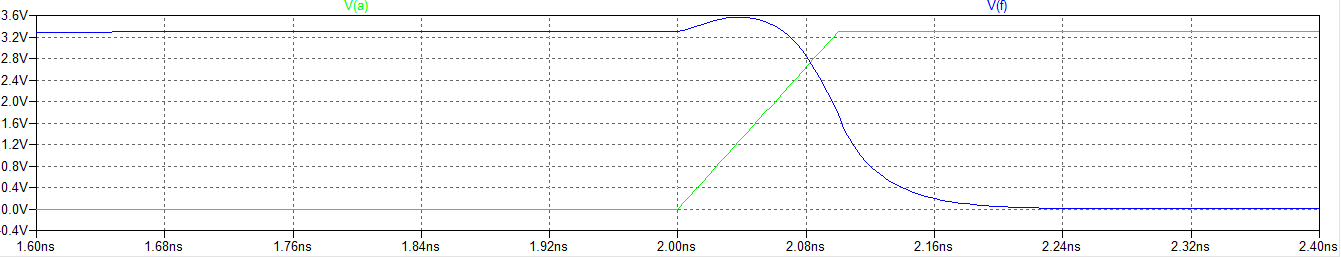
\includegraphics[scale=0.5]{./layout_mejor_graf.png}
    \rule{35em}{0.5pt}
  \caption[Captura]{Gráfica para mejor caso del NMOS en layout}
  \label{fig:layout_graf}
  \end{center}
\end{figure}

\section{Análisis de datos y resultados.}

El la Tabla \ref{table:TablaAnalitica} se muestran los valores del cálculo analítico de los delay de la compuerta para el mejor y peor caso de propagación de fall y raise, el mejor y peor caso para el delay de contaminación de raise y fall, estos por el método del delay de Elmore, así como el calculo del delay mediante el método del esfuerzo lógico.\\

A partir de esta tabla se puede observar que los cálculos del delay por medio del método de Elmore y por medio del metodo de esfuerzo logico son bastante cercanos, siendo el método de Elmore más complejo, pero permite un mejor análisis de los diferentes casos, necesario para un mejor diseño.\\

Conforme a los datos simulados experimentalmente, los tiempos de propagación de subida y bajada de los niveles lógicos sob aproximadamente cercanos pero no lo suficiente para ser simétricos. En comparación con la teoría de esfuerzo lógico, vemos que los valores son bastante aproximados.\\

Por último. Con la creación del layout fue bastante útil utilizar las técnicas del los caminos de Euler y el diagrama de palitos para crear el mismo. Vemos que al simular el layout, la gráfica muestra un mejor comportamiento a como se simuló en el esquemático.




\section{Conclusiones.}
\begin{itemize}
\item Los retardos de fall son mas lentos que los de rise, debido a la movilidad de los portadores presentes en cada red.
\item En el diseño de una compuerta, el método de esfuerzo lógico es necesario para poder dimensionar los transistores, mientras que el método de Elmore permite el análisis de los casos de delay de la compuerta.
\item La teoría del esfuerzo lógico y sus cálculos nos dán una buena aproximación para determinar una buena aproximación con los tiempos de retardo
\item Las técnicas de los caminos de Euler y el diseño del diagrama de palitos llega a ser muy útil para la creación de los layouts.

\end{itemize}

\section{Bibliografía}
%----------------------------------------------------------------------------------------
\begin{thebibliography}{3}

\bibliographystyle{unsrtnat} % Use the "unsrtnat" BibTeX style for formatting the Bibliography

\bibitem[Wey(1999)]{Wey1999}
[1] N. Weste, D. Harris. 
\newblock {CMOS VLSI Design: A Circuits and Systems Perspective , 4 edition.}.
\newblock \emph{Boston: Addison-Wesley}, 2010.

\bibitem[Wey(1999)]{Wey1999}
[2] J. Rabaey, A. Chandrakasan y B. Nikolic. 
\newblock { Digital Integrated Circuits: A Design Perspective.}.
\newblock \emph{Prentice Hall}, 2005.

\bibitem[Wey(1999)]{Wey1999}
[3]Test Data .On SemiconductorC5.Mosis. Recompilado de:
\newblock \emph{http://www.ie.itcr.ac.cr/achacon/ \\* Intro$\_Diseno\_CI/Modelos\_Spice\_$MOSIS/v03m-params.txt}, el 07/09/2015

\end{thebibliography}

\end{document}